\documentclass[1p]{elsarticle_modified}
%\bibliographystyle{elsarticle-num}

%\usepackage[colorlinks]{hyperref}
%\usepackage{abbrmath_seonhwa} %\Abb, \Ascr, \Acal ,\Abf, \Afrak
\usepackage{amsfonts}
\usepackage{amssymb}
\usepackage{amsmath}
\usepackage{amsthm}
\usepackage{scalefnt}
\usepackage{amsbsy}
\usepackage{kotex}
\usepackage{caption}
\usepackage{subfig}
\usepackage{color}
\usepackage{graphicx}
\usepackage{xcolor} %% white, black, red, green, blue, cyan, magenta, yellow
\usepackage{float}
\usepackage{setspace}
\usepackage{hyperref}

\usepackage{tikz}
\usetikzlibrary{arrows}

\usepackage{multirow}
\usepackage{array} % fixed length table
\usepackage{hhline}

%%%%%%%%%%%%%%%%%%%%%
\makeatletter
\renewcommand*\env@matrix[1][\arraystretch]{%
	\edef\arraystretch{#1}%
	\hskip -\arraycolsep
	\let\@ifnextchar\new@ifnextchar
	\array{*\c@MaxMatrixCols c}}
\makeatother %https://tex.stackexchange.com/questions/14071/how-can-i-increase-the-line-spacing-in-a-matrix
%%%%%%%%%%%%%%%

\usepackage[normalem]{ulem}

\newcommand{\msout}[1]{\ifmmode\text{\sout{\ensuremath{#1}}}\else\sout{#1}\fi}
%SOURCE: \msout is \stkout macro in https://tex.stackexchange.com/questions/20609/strikeout-in-math-mode

\newcommand{\cancel}[1]{
	\ifmmode
	{\color{red}\msout{#1}}
	\else
	{\color{red}\sout{#1}}
	\fi
}

\newcommand{\add}[1]{
	{\color{blue}\uwave{#1}}
}

\newcommand{\replace}[2]{
	\ifmmode
	{\color{red}\msout{#1}}{\color{blue}\uwave{#2}}
	\else
	{\color{red}\sout{#1}}{\color{blue}\uwave{#2}}
	\fi
}

\newcommand{\Sol}{\mathcal{S}} %segment
\newcommand{\D}{D} %diagram
\newcommand{\A}{\mathcal{A}} %arc


%%%%%%%%%%%%%%%%%%%%%%%%%%%%%5 test

\def\sl{\operatorname{\textup{SL}}(2,\Cbb)}
\def\psl{\operatorname{\textup{PSL}}(2,\Cbb)}
\def\quan{\mkern 1mu \triangleright \mkern 1mu}

\theoremstyle{definition}
\newtheorem{thm}{Theorem}[section]
\newtheorem{prop}[thm]{Proposition}
\newtheorem{lem}[thm]{Lemma}
\newtheorem{ques}[thm]{Question}
\newtheorem{cor}[thm]{Corollary}
\newtheorem{defn}[thm]{Definition}
\newtheorem{exam}[thm]{Example}
\newtheorem{rmk}[thm]{Remark}
\newtheorem{alg}[thm]{Algorithm}

\newcommand{\I}{\sqrt{-1}}
\begin{document}

%\begin{frontmatter}
%
%\title{Boundary parabolic representations of knots up to 8 crossings}
%
%%% Group authors per affiliation:
%\author{Yunhi Cho} 
%\address{Department of Mathematics, University of Seoul, Seoul, Korea}
%\ead{yhcho@uos.ac.kr}
%
%
%\author{Seonhwa Kim} %\fnref{s_kim}}
%\address{Center for Geometry and Physics, Institute for Basic Science, Pohang, 37673, Korea}
%\ead{ryeona17@ibs.re.kr}
%
%\author{Hyuk Kim}
%\address{Department of Mathematical Sciences, Seoul National University, Seoul 08826, Korea}
%\ead{hyukkim@snu.ac.kr}
%
%\author{Seokbeom Yoon}
%\address{Department of Mathematical Sciences, Seoul National University, Seoul, 08826,  Korea}
%\ead{sbyoon15@snu.ac.kr}
%
%\begin{abstract}
%We find all boundary parabolic representation of knots up to 8 crossings.
%
%\end{abstract}
%\begin{keyword}
%    \MSC[2010] 57M25 
%\end{keyword}
%
%\end{frontmatter}

%\linenumbers
%\tableofcontents
%
\newcommand\colored[1]{\textcolor{white}{\rule[-0.35ex]{0.8em}{1.4ex}}\kern-0.8em\color{red} #1}%
%\newcommand\colored[1]{\textcolor{white}{ #1}\kern-2.17ex	\textcolor{white}{ #1}\kern-1.81ex	\textcolor{white}{ #1}\kern-2.15ex\color{red}#1	}

{\Large $\underline{12n_{0241}~(K12n_{0241})}$}

\setlength{\tabcolsep}{10pt}
\renewcommand{\arraystretch}{1.6}
\vspace{1cm}\begin{tabular}{m{100pt}>{\centering\arraybackslash}m{274pt}}
\multirow{5}{120pt}{
	\centering
	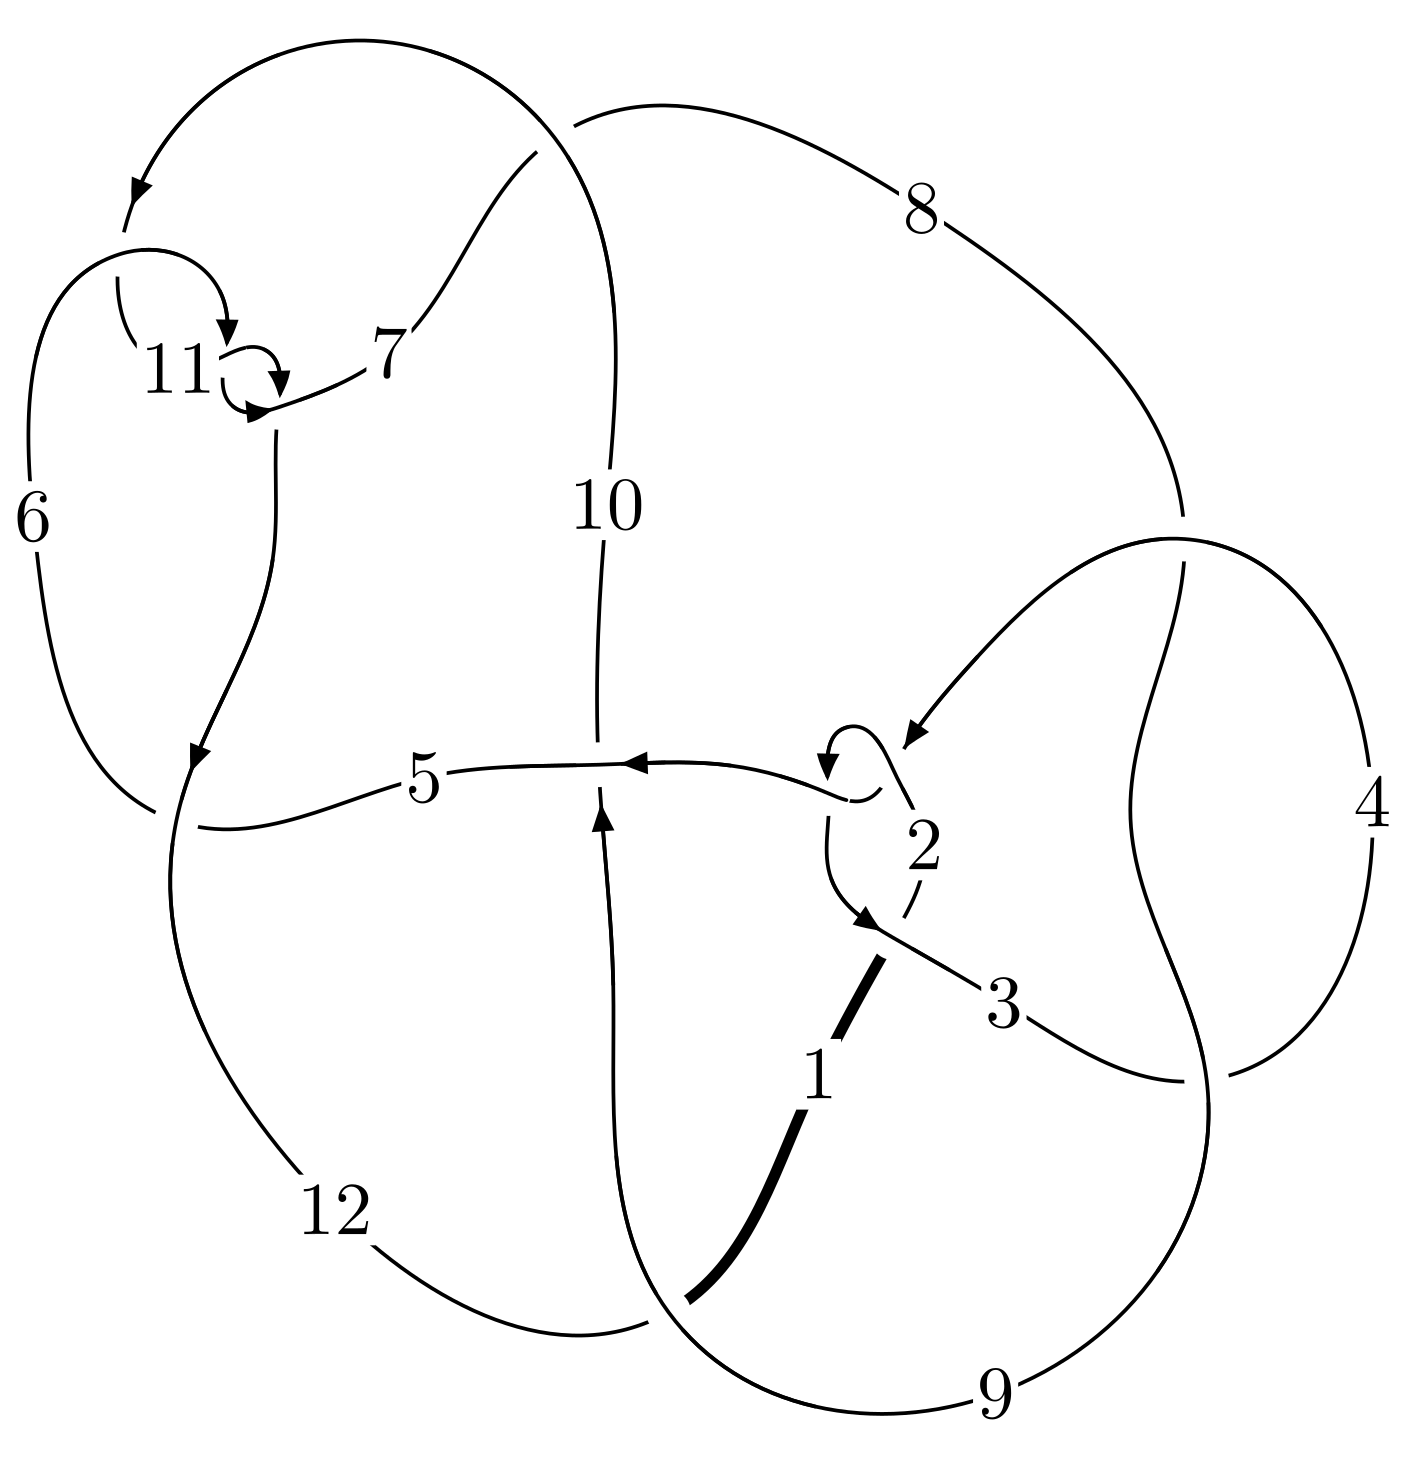
\includegraphics[width=112pt]{../../../GIT/diagram.site/Diagrams/png/2330_12n_0241.png}\\
\ \ \ A knot diagram\footnotemark}&
\allowdisplaybreaks
\textbf{Linearized knot diagam} \\
\cline{2-2}
 &
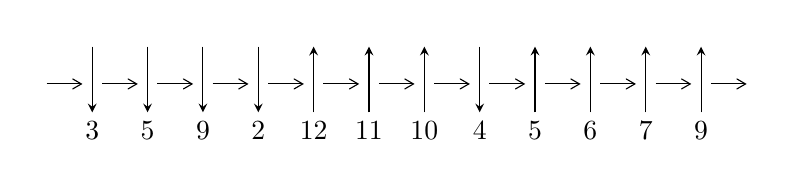
\begin{tikzpicture}[x=20pt, y=17pt]
	% nodes
	\node (C0) at (0, 0) {};
	\node (C1) at (1, 0) {};
	\node (C1U) at (1, +1) {};
	\node (C1D) at (1, -1) {3};

	\node (C2) at (2, 0) {};
	\node (C2U) at (2, +1) {};
	\node (C2D) at (2, -1) {5};

	\node (C3) at (3, 0) {};
	\node (C3U) at (3, +1) {};
	\node (C3D) at (3, -1) {9};

	\node (C4) at (4, 0) {};
	\node (C4U) at (4, +1) {};
	\node (C4D) at (4, -1) {2};

	\node (C5) at (5, 0) {};
	\node (C5U) at (5, +1) {};
	\node (C5D) at (5, -1) {12};

	\node (C6) at (6, 0) {};
	\node (C6U) at (6, +1) {};
	\node (C6D) at (6, -1) {11};

	\node (C7) at (7, 0) {};
	\node (C7U) at (7, +1) {};
	\node (C7D) at (7, -1) {10};

	\node (C8) at (8, 0) {};
	\node (C8U) at (8, +1) {};
	\node (C8D) at (8, -1) {4};

	\node (C9) at (9, 0) {};
	\node (C9U) at (9, +1) {};
	\node (C9D) at (9, -1) {5};

	\node (C10) at (10, 0) {};
	\node (C10U) at (10, +1) {};
	\node (C10D) at (10, -1) {6};

	\node (C11) at (11, 0) {};
	\node (C11U) at (11, +1) {};
	\node (C11D) at (11, -1) {7};

	\node (C12) at (12, 0) {};
	\node (C12U) at (12, +1) {};
	\node (C12D) at (12, -1) {9};
	\node (C13) at (13, 0) {};

	% arrows
	\draw[->,>={angle 60}]
	(C0) edge (C1) (C1) edge (C2) (C2) edge (C3) (C3) edge (C4) (C4) edge (C5) (C5) edge (C6) (C6) edge (C7) (C7) edge (C8) (C8) edge (C9) (C9) edge (C10) (C10) edge (C11) (C11) edge (C12) (C12) edge (C13) ;	\draw[->,>=stealth]
	(C1U) edge (C1D) (C2U) edge (C2D) (C3U) edge (C3D) (C4U) edge (C4D) (C5D) edge (C5U) (C6D) edge (C6U) (C7D) edge (C7U) (C8U) edge (C8D) (C9D) edge (C9U) (C10D) edge (C10U) (C11D) edge (C11U) (C12D) edge (C12U) ;
	\end{tikzpicture} \\
\hhline{~~} \\& 
\textbf{Solving Sequence} \\ \cline{2-2} 
 &
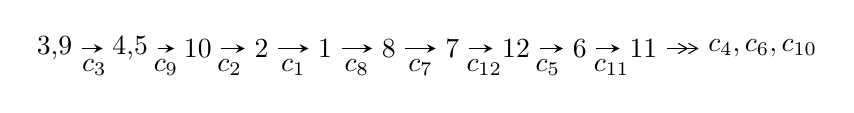
\begin{tikzpicture}[x=23pt, y=7pt]
	% node
	\node (A0) at (-1/8, 0) {3,9};
	\node (A1) at (17/16, 0) {4,5};
	\node (A2) at (17/8, 0) {10};
	\node (A3) at (25/8, 0) {2};
	\node (A4) at (33/8, 0) {1};
	\node (A5) at (41/8, 0) {8};
	\node (A6) at (49/8, 0) {7};
	\node (A7) at (57/8, 0) {12};
	\node (A8) at (65/8, 0) {6};
	\node (A9) at (73/8, 0) {11};
	\node (C1) at (1/2, -1) {$c_{3}$};
	\node (C2) at (13/8, -1) {$c_{9}$};
	\node (C3) at (21/8, -1) {$c_{2}$};
	\node (C4) at (29/8, -1) {$c_{1}$};
	\node (C5) at (37/8, -1) {$c_{8}$};
	\node (C6) at (45/8, -1) {$c_{7}$};
	\node (C7) at (53/8, -1) {$c_{12}$};
	\node (C8) at (61/8, -1) {$c_{5}$};
	\node (C9) at (69/8, -1) {$c_{11}$};
	\node (A10) at (11, 0) {$c_{4},c_{6},c_{10}$};

	% edge
	\draw[->,>=stealth]	
	(A0) edge (A1) (A1) edge (A2) (A2) edge (A3) (A3) edge (A4) (A4) edge (A5) (A5) edge (A6) (A6) edge (A7) (A7) edge (A8) (A8) edge (A9) ;
	\draw[->>,>={angle 60}]	
	(A9) edge (A10);
\end{tikzpicture} \\ 

\end{tabular} \\

\footnotetext{
The image of knot diagram is generated by the software ``\textbf{Draw programme}" developed by Andrew Bartholomew(\url{http://www.layer8.co.uk/maths/draw/index.htm\#Running-draw}), where we modified some parts for our purpose(\url{https://github.com/CATsTAILs/LinksPainter}).
}\phantom \\ \newline 
\centering \textbf{Ideals for irreducible components\footnotemark of $X_{\text{par}}$} 
 
\begin{align*}
I^u_{1}&=\langle 
-1.03137\times10^{66} u^{36}+6.98280\times10^{65} u^{35}+\cdots+2.95081\times10^{68} b-1.06268\times10^{68},\\
\phantom{I^u_{1}}&\phantom{= \langle  }3.77823\times10^{67} u^{36}-2.87660\times10^{67} u^{35}+\cdots+2.36065\times10^{69} a+2.08922\times10^{69},\\
\phantom{I^u_{1}}&\phantom{= \langle  }u^{37}- u^{36}+\cdots+128 u+256\rangle \\
\\
I^v_{1}&=\langle 
a,\;b-1,\;v^8- v^7- v^6+2 v^5+v^4-2 v^3+2 v-1\rangle \\
\end{align*}
\raggedright * 2 irreducible components of $\dim_{\mathbb{C}}=0$, with total 45 representations.\\
\footnotetext{All coefficients of polynomials are rational numbers. But the coefficients are sometimes approximated in decimal forms when there is not enough margin.}
\newpage
\renewcommand{\arraystretch}{1}
\centering \section*{I. $I^u_{1}= \langle -1.03\times10^{66} u^{36}+6.98\times10^{65} u^{35}+\cdots+2.95\times10^{68} b-1.06\times10^{68},\;3.78\times10^{67} u^{36}-2.88\times10^{67} u^{35}+\cdots+2.36\times10^{69} a+2.09\times10^{69},\;u^{37}- u^{36}+\cdots+128 u+256 \rangle$}
\flushleft \textbf{(i) Arc colorings}\\
\begin{tabular}{m{7pt} m{180pt} m{7pt} m{180pt} }
\flushright $a_{3}=$&$\begin{pmatrix}1\\0\end{pmatrix}$ \\
\flushright $a_{9}=$&$\begin{pmatrix}0\\u\end{pmatrix}$ \\
\flushright $a_{4}=$&$\begin{pmatrix}1\\u^2\end{pmatrix}$ \\
\flushright $a_{5}=$&$\begin{pmatrix}-0.0160050 u^{36}+0.0121856 u^{35}+\cdots-8.06518 u-0.885020\\0.00349520 u^{36}-0.00236640 u^{35}+\cdots+1.79889 u+0.360133\end{pmatrix}$ \\
\flushright $a_{10}=$&$\begin{pmatrix}-0.0133199 u^{36}+0.0418348 u^{35}+\cdots+0.507839 u+12.6265\\0.00381941 u^{36}-0.0132824 u^{35}+\cdots+0.836374 u-4.09729\end{pmatrix}$ \\
\flushright $a_{2}=$&$\begin{pmatrix}-0.0160050 u^{36}+0.0121856 u^{35}+\cdots-8.06518 u-0.885020\\0.00596782 u^{36}-0.00520306 u^{35}+\cdots+2.78728 u+0.617635\end{pmatrix}$ \\
\flushright $a_{1}=$&$\begin{pmatrix}-0.0100372 u^{36}+0.00698258 u^{35}+\cdots-5.27790 u-0.267385\\0.00596782 u^{36}-0.00520306 u^{35}+\cdots+2.78728 u+0.617635\end{pmatrix}$ \\
\flushright $a_{8}=$&$\begin{pmatrix}u\\u^3+u\end{pmatrix}$ \\
\flushright $a_{7}=$&$\begin{pmatrix}-0.0154489 u^{36}+0.0231599 u^{35}+\cdots-4.79943 u+5.30651\\-0.000302840 u^{36}+0.00840424 u^{35}+\cdots+2.35144 u+2.54004\end{pmatrix}$ \\
\flushright $a_{12}=$&$\begin{pmatrix}-0.0100372 u^{36}+0.00698258 u^{35}+\cdots-5.27790 u-0.267385\\0.0110751 u^{36}-0.00839995 u^{35}+\cdots+5.74781 u+1.39963\end{pmatrix}$ \\
\flushright $a_{6}=$&$\begin{pmatrix}-0.0440610 u^{36}+0.0321408 u^{35}+\cdots-23.2326 u-5.35412\\0.0221974 u^{36}-0.0147892 u^{35}+\cdots+12.6696 u+3.48847\end{pmatrix}$ \\
\flushright $a_{11}=$&$\begin{pmatrix}-0.0148066 u^{36}+0.00829427 u^{35}+\cdots-11.4914 u-1.08615\\-0.00186082 u^{36}+0.00671544 u^{35}+\cdots+3.81289 u+3.67874\end{pmatrix}$\\&\end{tabular}
\flushleft \textbf{(ii) Obstruction class $= -1$}\\~\\
\flushleft \textbf{(iii) Cusp Shapes $= -0.0751690 u^{36}+0.0952069 u^{35}+\cdots-23.9143 u+7.79267$}\\~\\
\newpage\renewcommand{\arraystretch}{1}
\flushleft \textbf{(iv) u-Polynomials at the component}\newline \\
\begin{tabular}{m{50pt}|m{274pt}}
Crossings & \hspace{64pt}u-Polynomials at each crossing \\
\hline $$\begin{aligned}c_{1}\end{aligned}$$&$\begin{aligned}
&u^{37}+5 u^{36}+\cdots-5 u+1
\end{aligned}$\\
\hline $$\begin{aligned}c_{2},c_{4}\end{aligned}$$&$\begin{aligned}
&u^{37}-9 u^{36}+\cdots-7 u+1
\end{aligned}$\\
\hline $$\begin{aligned}c_{3},c_{8}\end{aligned}$$&$\begin{aligned}
&u^{37}- u^{36}+\cdots+128 u+256
\end{aligned}$\\
\hline $$\begin{aligned}c_{5},c_{7}\end{aligned}$$&$\begin{aligned}
&u^{37}+6 u^{36}+\cdots+35 u+5
\end{aligned}$\\
\hline $$\begin{aligned}c_{6},c_{10},c_{11}\end{aligned}$$&$\begin{aligned}
&u^{37}-2 u^{36}+\cdots+3 u+1
\end{aligned}$\\
\hline $$\begin{aligned}c_{9}\end{aligned}$$&$\begin{aligned}
&u^{37}+2 u^{36}+\cdots+3 u+1
\end{aligned}$\\
\hline $$\begin{aligned}c_{12}\end{aligned}$$&$\begin{aligned}
&u^{37}-8 u^{36}+\cdots+2082719 u-154033
\end{aligned}$\\
\hline
\end{tabular}\\~\\
\newpage\renewcommand{\arraystretch}{1}
\flushleft \textbf{(v) Riley Polynomials at the component}\newline \\
\begin{tabular}{m{50pt}|m{274pt}}
Crossings & \hspace{64pt}Riley Polynomials at each crossing \\
\hline $$\begin{aligned}c_{1}\end{aligned}$$&$\begin{aligned}
&y^{37}+63 y^{36}+\cdots- y-1
\end{aligned}$\\
\hline $$\begin{aligned}c_{2},c_{4}\end{aligned}$$&$\begin{aligned}
&y^{37}-5 y^{36}+\cdots-5 y-1
\end{aligned}$\\
\hline $$\begin{aligned}c_{3},c_{8}\end{aligned}$$&$\begin{aligned}
&y^{37}+51 y^{36}+\cdots-475136 y-65536
\end{aligned}$\\
\hline $$\begin{aligned}c_{5},c_{7}\end{aligned}$$&$\begin{aligned}
&y^{37}+16 y^{36}+\cdots+735 y-25
\end{aligned}$\\
\hline $$\begin{aligned}c_{6},c_{10},c_{11}\end{aligned}$$&$\begin{aligned}
&y^{37}-32 y^{36}+\cdots+27 y-1
\end{aligned}$\\
\hline $$\begin{aligned}c_{9}\end{aligned}$$&$\begin{aligned}
&y^{37}-48 y^{36}+\cdots+27 y-1
\end{aligned}$\\
\hline $$\begin{aligned}c_{12}\end{aligned}$$&$\begin{aligned}
&y^{37}-84 y^{36}+\cdots+1848165923715 y-23726165089
\end{aligned}$\\
\hline
\end{tabular}\\~\\
\newpage\flushleft \textbf{(vi) Complex Volumes and Cusp Shapes}
$$\begin{array}{c|c|c}  
\text{Solutions to }I^u_{1}& \I (\text{vol} + \sqrt{-1}CS) & \text{Cusp shape}\\
 \hline 
\begin{aligned}
u &= -0.878368 + 0.497461 I \\
a &= \phantom{-}0.626443 + 0.343621 I \\
b &= \phantom{-}0.227102 - 0.673098 I\end{aligned}
 & -0.66892 + 2.27408 I & \phantom{-}1.99793 - 4.76069 I \\ \hline\begin{aligned}
u &= -0.878368 - 0.497461 I \\
a &= \phantom{-}0.626443 - 0.343621 I \\
b &= \phantom{-}0.227102 + 0.673098 I\end{aligned}
 & -0.66892 - 2.27408 I & \phantom{-}1.99793 + 4.76069 I \\ \hline\begin{aligned}
u &= -0.756357 + 0.569885 I \\
a &= \phantom{-}0.466384 - 0.081501 I \\
b &= \phantom{-}1.080620 + 0.363590 I\end{aligned}
 & \phantom{-}0.61705 - 4.41139 I & \phantom{-}2.87485 + 3.50022 I \\ \hline\begin{aligned}
u &= -0.756357 - 0.569885 I \\
a &= \phantom{-}0.466384 + 0.081501 I \\
b &= \phantom{-}1.080620 - 0.363590 I\end{aligned}
 & \phantom{-}0.61705 + 4.41139 I & \phantom{-}2.87485 - 3.50022 I \\ \hline\begin{aligned}
u &= -0.491761 + 0.952107 I \\
a &= \phantom{-}0.695040 + 0.682945 I \\
b &= -0.267990 - 0.719272 I\end{aligned}
 & \phantom{-}6.82750 - 1.30632 I & \phantom{-}10.37535 + 1.68426 I \\ \hline\begin{aligned}
u &= -0.491761 - 0.952107 I \\
a &= \phantom{-}0.695040 - 0.682945 I \\
b &= -0.267990 + 0.719272 I\end{aligned}
 & \phantom{-}6.82750 + 1.30632 I & \phantom{-}10.37535 - 1.68426 I \\ \hline\begin{aligned}
u &= \phantom{-}0.886724 + 0.087993 I \\
a &= \phantom{-}0.586081 - 0.184026 I \\
b &= \phantom{-}0.553122 + 0.487673 I\end{aligned}
 & \phantom{-}2.29551 + 0.52381 I & \phantom{-}5.03075 + 0.94889 I \\ \hline\begin{aligned}
u &= \phantom{-}0.886724 - 0.087993 I \\
a &= \phantom{-}0.586081 + 0.184026 I \\
b &= \phantom{-}0.553122 - 0.487673 I\end{aligned}
 & \phantom{-}2.29551 - 0.52381 I & \phantom{-}5.03075 - 0.94889 I \\ \hline\begin{aligned}
u &= -0.366615 + 0.752594 I \\
a &= \phantom{-}0.451654 - 0.034286 I \\
b &= \phantom{-}1.201400 + 0.167112 I\end{aligned}
 & \phantom{-}0.11703 + 2.14687 I & \phantom{-}4.21868 - 4.14096 I \\ \hline\begin{aligned}
u &= -0.366615 - 0.752594 I \\
a &= \phantom{-}0.451654 + 0.034286 I \\
b &= \phantom{-}1.201400 - 0.167112 I\end{aligned}
 & \phantom{-}0.11703 - 2.14687 I & \phantom{-}4.21868 + 4.14096 I\\
 \hline 
 \end{array}$$\newpage$$\begin{array}{c|c|c}  
\text{Solutions to }I^u_{1}& \I (\text{vol} + \sqrt{-1}CS) & \text{Cusp shape}\\
 \hline 
\begin{aligned}
u &= \phantom{-}0.040136 + 0.830344 I \\
a &= \phantom{-}1.19957 - 1.19424 I \\
b &= -0.581327 + 0.416814 I\end{aligned}
 & \phantom{-}1.73939 + 7.30260 I & \phantom{-}6.40314 - 7.32057 I \\ \hline\begin{aligned}
u &= \phantom{-}0.040136 - 0.830344 I \\
a &= \phantom{-}1.19957 + 1.19424 I \\
b &= -0.581327 - 0.416814 I\end{aligned}
 & \phantom{-}1.73939 - 7.30260 I & \phantom{-}6.40314 + 7.32057 I \\ \hline\begin{aligned}
u &= \phantom{-}0.563224 + 0.605095 I \\
a &= \phantom{-}0.466156 + 0.056547 I \\
b &= \phantom{-}1.114100 - 0.256450 I\end{aligned}
 & -3.61155 + 1.05730 I & -2.65114 + 0.19593 I \\ \hline\begin{aligned}
u &= \phantom{-}0.563224 - 0.605095 I \\
a &= \phantom{-}0.466156 - 0.056547 I \\
b &= \phantom{-}1.114100 + 0.256450 I\end{aligned}
 & -3.61155 - 1.05730 I & -2.65114 - 0.19593 I \\ \hline\begin{aligned}
u &= \phantom{-}0.981996 + 0.654437 I \\
a &= \phantom{-}0.572407 - 0.396675 I \\
b &= \phantom{-}0.180218 + 0.817886 I\end{aligned}
 & \phantom{-}4.10036 - 5.71187 I & \phantom{-}7.23097 + 5.43034 I \\ \hline\begin{aligned}
u &= \phantom{-}0.981996 - 0.654437 I \\
a &= \phantom{-}0.572407 + 0.396675 I \\
b &= \phantom{-}0.180218 - 0.817886 I\end{aligned}
 & \phantom{-}4.10036 + 5.71187 I & \phantom{-}7.23097 - 5.43034 I \\ \hline\begin{aligned}
u &= -0.066568 + 0.771395 I \\
a &= \phantom{-}1.33592 + 1.03307 I \\
b &= -0.531570 - 0.362239 I\end{aligned}
 & -2.71712 - 3.28265 I & \phantom{-}1.87410 + 4.96573 I \\ \hline\begin{aligned}
u &= -0.066568 - 0.771395 I \\
a &= \phantom{-}1.33592 - 1.03307 I \\
b &= -0.531570 + 0.362239 I\end{aligned}
 & -2.71712 + 3.28265 I & \phantom{-}1.87410 - 4.96573 I \\ \hline\begin{aligned}
u &= \phantom{-}0.419103 + 0.595983 I \\
a &= \phantom{-}0.910599 - 0.447643 I \\
b &= -0.115558 + 0.434784 I\end{aligned}
 & \phantom{-}1.109940 + 0.478757 I & \phantom{-}7.85612 - 2.59030 I \\ \hline\begin{aligned}
u &= \phantom{-}0.419103 - 0.595983 I \\
a &= \phantom{-}0.910599 + 0.447643 I \\
b &= -0.115558 - 0.434784 I\end{aligned}
 & \phantom{-}1.109940 - 0.478757 I & \phantom{-}7.85612 + 2.59030 I\\
 \hline 
 \end{array}$$\newpage$$\begin{array}{c|c|c}  
\text{Solutions to }I^u_{1}& \I (\text{vol} + \sqrt{-1}CS) & \text{Cusp shape}\\
 \hline 
\begin{aligned}
u &= \phantom{-}0.077849 + 0.690240 I \\
a &= \phantom{-}1.50612 - 0.77029 I \\
b &= -0.473705 + 0.269170 I\end{aligned}
 & \phantom{-}0.539059 - 0.667337 I & \phantom{-}5.56096 - 0.61157 I \\ \hline\begin{aligned}
u &= \phantom{-}0.077849 - 0.690240 I \\
a &= \phantom{-}1.50612 + 0.77029 I \\
b &= -0.473705 - 0.269170 I\end{aligned}
 & \phantom{-}0.539059 + 0.667337 I & \phantom{-}5.56096 + 0.61157 I \\ \hline\begin{aligned}
u &= -0.407194\phantom{ +0.000000I} \\
a &= \phantom{-}0.525318\phantom{ +0.000000I} \\
b &= \phantom{-}0.903607\phantom{ +0.000000I}\end{aligned}
 & -1.31151\phantom{ +0.000000I} & -10.2650\phantom{ +0.000000I} \\ \hline\begin{aligned}
u &= \phantom{-}0.39124 + 1.82665 I \\
a &= -0.068005 + 0.975912 I \\
b &= -1.07106 - 1.01973 I\end{aligned}
 & \phantom{-}9.29659 - 4.13983 I & \phantom{-0.000000 } 0 \\ \hline\begin{aligned}
u &= \phantom{-}0.39124 - 1.82665 I \\
a &= -0.068005 - 0.975912 I \\
b &= -1.07106 + 1.01973 I\end{aligned}
 & \phantom{-}9.29659 + 4.13983 I & \phantom{-0.000000 } 0 \\ \hline\begin{aligned}
u &= \phantom{-}0.24251 + 1.87487 I \\
a &= \phantom{-}0.000094 + 0.931629 I \\
b &= -0.99989 - 1.07339 I\end{aligned}
 & \phantom{-}9.54816 - 3.51968 I & \phantom{-0.000000 } 0 \\ \hline\begin{aligned}
u &= \phantom{-}0.24251 - 1.87487 I \\
a &= \phantom{-}0.000094 - 0.931629 I \\
b &= -0.99989 + 1.07339 I\end{aligned}
 & \phantom{-}9.54816 + 3.51968 I & \phantom{-0.000000 } 0 \\ \hline\begin{aligned}
u &= -0.48778 + 1.83564 I \\
a &= -0.120525 - 0.976988 I \\
b &= -1.12438 + 1.00821 I\end{aligned}
 & \phantom{-}6.99297 + 8.38148 I & \phantom{-0.000000 } 0 \\ \hline\begin{aligned}
u &= -0.48778 - 1.83564 I \\
a &= -0.120525 + 0.976988 I \\
b &= -1.12438 - 1.00821 I\end{aligned}
 & \phantom{-}6.99297 - 8.38148 I & \phantom{-0.000000 } 0 \\ \hline\begin{aligned}
u &= -0.13124 + 1.93107 I \\
a &= \phantom{-}0.037828 - 0.886275 I \\
b &= -0.95193 + 1.12627 I\end{aligned}
 & \phantom{-}7.58072 - 0.60625 I & \phantom{-0.000000 } 0\\
 \hline 
 \end{array}$$\newpage$$\begin{array}{c|c|c}  
\text{Solutions to }I^u_{1}& \I (\text{vol} + \sqrt{-1}CS) & \text{Cusp shape}\\
 \hline 
\begin{aligned}
u &= -0.13124 - 1.93107 I \\
a &= \phantom{-}0.037828 + 0.886275 I \\
b &= -0.95193 - 1.12627 I\end{aligned}
 & \phantom{-}7.58072 + 0.60625 I & \phantom{-0.000000 } 0 \\ \hline\begin{aligned}
u &= \phantom{-}0.53822 + 1.86696 I \\
a &= -0.147624 + 0.960917 I \\
b &= -1.15619 - 1.01668 I\end{aligned}
 & \phantom{-}12.0430 - 12.4368 I & \phantom{-0.000000 } 0 \\ \hline\begin{aligned}
u &= \phantom{-}0.53822 - 1.86696 I \\
a &= -0.147624 - 0.960917 I \\
b &= -1.15619 + 1.01668 I\end{aligned}
 & \phantom{-}12.0430 + 12.4368 I & \phantom{-0.000000 } 0 \\ \hline\begin{aligned}
u &= \phantom{-}0.09684 + 2.00647 I \\
a &= \phantom{-}0.036196 + 0.850721 I \\
b &= -0.95008 - 1.17335 I\end{aligned}
 & \phantom{-}12.76300 + 4.48472 I & \phantom{-0.000000 } 0 \\ \hline\begin{aligned}
u &= \phantom{-}0.09684 - 2.00647 I \\
a &= \phantom{-}0.036196 - 0.850721 I \\
b &= -0.95008 + 1.17335 I\end{aligned}
 & \phantom{-}12.76300 - 4.48472 I & \phantom{-0.000000 } 0 \\ \hline\begin{aligned}
u &= -0.35556 + 2.00636 I \\
a &= -0.066983 - 0.886854 I \\
b &= -1.08468 + 1.12119 I\end{aligned}
 & \phantom{-}16.7972 + 4.0807 I & \phantom{-0.000000 } 0 \\ \hline\begin{aligned}
u &= -0.35556 - 2.00636 I \\
a &= -0.066983 + 0.886854 I \\
b &= -1.08468 - 1.12119 I\end{aligned}
 & \phantom{-}16.7972 - 4.0807 I & \phantom{-0.000000 } 0\\
 \hline 
 \end{array}$$\newpage\newpage\renewcommand{\arraystretch}{1}
\centering \section*{II. $I^v_{1}= \langle a,\;b-1,\;v^8- v^7- v^6+2 v^5+v^4-2 v^3+2 v-1 \rangle$}
\flushleft \textbf{(i) Arc colorings}\\
\begin{tabular}{m{7pt} m{180pt} m{7pt} m{180pt} }
\flushright $a_{3}=$&$\begin{pmatrix}1\\0\end{pmatrix}$ \\
\flushright $a_{9}=$&$\begin{pmatrix}v\\0\end{pmatrix}$ \\
\flushright $a_{4}=$&$\begin{pmatrix}1\\0\end{pmatrix}$ \\
\flushright $a_{5}=$&$\begin{pmatrix}0\\1\end{pmatrix}$ \\
\flushright $a_{10}=$&$\begin{pmatrix}v\\- v\end{pmatrix}$ \\
\flushright $a_{2}=$&$\begin{pmatrix}1\\-1\end{pmatrix}$ \\
\flushright $a_{1}=$&$\begin{pmatrix}0\\-1\end{pmatrix}$ \\
\flushright $a_{8}=$&$\begin{pmatrix}v\\0\end{pmatrix}$ \\
\flushright $a_{7}=$&$\begin{pmatrix}- v^3+v\\v^3\end{pmatrix}$ \\
\flushright $a_{12}=$&$\begin{pmatrix}v^2\\-1\end{pmatrix}$ \\
\flushright $a_{6}=$&$\begin{pmatrix}v^4\\- v^2+1\end{pmatrix}$ \\
\flushright $a_{11}=$&$\begin{pmatrix}- v^7+v^6+2 v^5- v^4-2 v^3+2 v^2+2 v-1\\v^7-2 v^5+2 v^3-2 v\end{pmatrix}$\\&\end{tabular}
\flushleft \textbf{(ii) Obstruction class $= 1$}\\~\\
\flushleft \textbf{(iii) Cusp Shapes $= 6 v^7- v^6-11 v^5+7 v^4+12 v^3-6 v^2-6 v+10$}\\~\\
\newpage\renewcommand{\arraystretch}{1}
\flushleft \textbf{(iv) u-Polynomials at the component}\newline \\
\begin{tabular}{m{50pt}|m{274pt}}
Crossings & \hspace{64pt}u-Polynomials at each crossing \\
\hline $$\begin{aligned}c_{1},c_{2}\end{aligned}$$&$\begin{aligned}
&(u-1)^8
\end{aligned}$\\
\hline $$\begin{aligned}c_{3},c_{8}\end{aligned}$$&$\begin{aligned}
&u^8
\end{aligned}$\\
\hline $$\begin{aligned}c_{4}\end{aligned}$$&$\begin{aligned}
&(u+1)^8
\end{aligned}$\\
\hline $$\begin{aligned}c_{5},c_{7}\end{aligned}$$&$\begin{aligned}
&u^8+3 u^7+7 u^6+10 u^5+11 u^4+10 u^3+6 u^2+4 u+1
\end{aligned}$\\
\hline $$\begin{aligned}c_{6}\end{aligned}$$&$\begin{aligned}
&u^8- u^7-3 u^6+2 u^5+3 u^4-2 u-1
\end{aligned}$\\
\hline $$\begin{aligned}c_{9},c_{12}\end{aligned}$$&$\begin{aligned}
&u^8- u^7- u^6+2 u^5+u^4-2 u^3+2 u-1
\end{aligned}$\\
\hline $$\begin{aligned}c_{10},c_{11}\end{aligned}$$&$\begin{aligned}
&u^8+u^7-3 u^6-2 u^5+3 u^4+2 u-1
\end{aligned}$\\
\hline
\end{tabular}\\~\\
\newpage\renewcommand{\arraystretch}{1}
\flushleft \textbf{(v) Riley Polynomials at the component}\newline \\
\begin{tabular}{m{50pt}|m{274pt}}
Crossings & \hspace{64pt}Riley Polynomials at each crossing \\
\hline $$\begin{aligned}c_{1},c_{2},c_{4}\end{aligned}$$&$\begin{aligned}
&(y-1)^8
\end{aligned}$\\
\hline $$\begin{aligned}c_{3},c_{8}\end{aligned}$$&$\begin{aligned}
&y^8
\end{aligned}$\\
\hline $$\begin{aligned}c_{5},c_{7}\end{aligned}$$&$\begin{aligned}
&y^8+5 y^7+11 y^6+6 y^5-17 y^4-34 y^3-22 y^2-4 y+1
\end{aligned}$\\
\hline $$\begin{aligned}c_{6},c_{10},c_{11}\end{aligned}$$&$\begin{aligned}
&y^8-7 y^7+19 y^6-22 y^5+3 y^4+14 y^3-6 y^2-4 y+1
\end{aligned}$\\
\hline $$\begin{aligned}c_{9},c_{12}\end{aligned}$$&$\begin{aligned}
&y^8-3 y^7+7 y^6-10 y^5+11 y^4-10 y^3+6 y^2-4 y+1
\end{aligned}$\\
\hline
\end{tabular}\\~\\
\newpage\flushleft \textbf{(vi) Complex Volumes and Cusp Shapes}
$$\begin{array}{c|c|c}  
\text{Solutions to }I^v_{1}& \I (\text{vol} + \sqrt{-1}CS) & \text{Cusp shape}\\
 \hline 
\begin{aligned}
v &= \phantom{-}0.570868 + 0.730671 I \\
a &= \phantom{-0.000000 } 0 \\
b &= \phantom{-}1.00000\phantom{ +0.000000I}\end{aligned}
 & -0.604279 - 1.131230 I & -1.074136 + 0.216470 I \\ \hline\begin{aligned}
v &= \phantom{-}0.570868 - 0.730671 I \\
a &= \phantom{-0.000000 } 0 \\
b &= \phantom{-}1.00000\phantom{ +0.000000I}\end{aligned}
 & -0.604279 + 1.131230 I & -1.074136 - 0.216470 I \\ \hline\begin{aligned}
v &= -0.855237 + 0.665892 I \\
a &= \phantom{-0.000000 } 0 \\
b &= \phantom{-}1.00000\phantom{ +0.000000I}\end{aligned}
 & -3.80435 - 2.57849 I & -3.22623 + 3.25417 I \\ \hline\begin{aligned}
v &= -0.855237 - 0.665892 I \\
a &= \phantom{-0.000000 } 0 \\
b &= \phantom{-}1.00000\phantom{ +0.000000I}\end{aligned}
 & -3.80435 + 2.57849 I & -3.22623 - 3.25417 I \\ \hline\begin{aligned}
v &= -1.09818\phantom{ +0.000000I} \\
a &= \phantom{-0.000000 } 0 \\
b &= \phantom{-}1.00000\phantom{ +0.000000I}\end{aligned}
 & \phantom{-}4.85780\phantom{ +0.000000I} & \phantom{-}7.89920\phantom{ +0.000000I} \\ \hline\begin{aligned}
v &= \phantom{-}1.031810 + 0.655470 I \\
a &= \phantom{-0.000000 } 0 \\
b &= \phantom{-}1.00000\phantom{ +0.000000I}\end{aligned}
 & \phantom{-}0.73474 + 6.44354 I & \phantom{-}2.34782 - 4.54733 I \\ \hline\begin{aligned}
v &= \phantom{-}1.031810 - 0.655470 I \\
a &= \phantom{-0.000000 } 0 \\
b &= \phantom{-}1.00000\phantom{ +0.000000I}\end{aligned}
 & \phantom{-}0.73474 - 6.44354 I & \phantom{-}2.34782 + 4.54733 I \\ \hline\begin{aligned}
v &= \phantom{-}0.603304\phantom{ +0.000000I} \\
a &= \phantom{-0.000000 } 0 \\
b &= \phantom{-}1.00000\phantom{ +0.000000I}\end{aligned}
 & -0.799899\phantom{ +0.000000I} & \phantom{-}7.00590\phantom{ +0.000000I}\\
 \hline 
 \end{array}$$\newpage
\newpage\renewcommand{\arraystretch}{1}
\centering \section*{ III. u-Polynomials}
\begin{tabular}{m{50pt}|m{274pt}}
Crossings & \hspace{64pt}u-Polynomials at each crossing \\
\hline $$\begin{aligned}c_{1}\end{aligned}$$&$\begin{aligned}
&((u-1)^8)(u^{37}+5 u^{36}+\cdots-5 u+1)
\end{aligned}$\\
\hline $$\begin{aligned}c_{2}\end{aligned}$$&$\begin{aligned}
&((u-1)^8)(u^{37}-9 u^{36}+\cdots-7 u+1)
\end{aligned}$\\
\hline $$\begin{aligned}c_{3},c_{8}\end{aligned}$$&$\begin{aligned}
&u^8(u^{37}- u^{36}+\cdots+128 u+256)
\end{aligned}$\\
\hline $$\begin{aligned}c_{4}\end{aligned}$$&$\begin{aligned}
&((u+1)^8)(u^{37}-9 u^{36}+\cdots-7 u+1)
\end{aligned}$\\
\hline $$\begin{aligned}c_{5},c_{7}\end{aligned}$$&$\begin{aligned}
&(u^8+3 u^7+7 u^6+10 u^5+11 u^4+10 u^3+6 u^2+4 u+1)\\
&\cdot(u^{37}+6 u^{36}+\cdots+35 u+5)
\end{aligned}$\\
\hline $$\begin{aligned}c_{6}\end{aligned}$$&$\begin{aligned}
&(u^8- u^7-3 u^6+2 u^5+3 u^4-2 u-1)(u^{37}-2 u^{36}+\cdots+3 u+1)
\end{aligned}$\\
\hline $$\begin{aligned}c_{9}\end{aligned}$$&$\begin{aligned}
&(u^8- u^7+\cdots+2 u-1)(u^{37}+2 u^{36}+\cdots+3 u+1)
\end{aligned}$\\
\hline $$\begin{aligned}c_{10},c_{11}\end{aligned}$$&$\begin{aligned}
&(u^8+u^7-3 u^6-2 u^5+3 u^4+2 u-1)(u^{37}-2 u^{36}+\cdots+3 u+1)
\end{aligned}$\\
\hline $$\begin{aligned}c_{12}\end{aligned}$$&$\begin{aligned}
&(u^8- u^7- u^6+2 u^5+u^4-2 u^3+2 u-1)\\
&\cdot(u^{37}-8 u^{36}+\cdots+2082719 u-154033)
\end{aligned}$\\
\hline
\end{tabular}\newpage\renewcommand{\arraystretch}{1}
\centering \section*{ IV. Riley Polynomials}
\begin{tabular}{m{50pt}|m{274pt}}
Crossings & \hspace{64pt}Riley Polynomials at each crossing \\
\hline $$\begin{aligned}c_{1}\end{aligned}$$&$\begin{aligned}
&((y-1)^8)(y^{37}+63 y^{36}+\cdots- y-1)
\end{aligned}$\\
\hline $$\begin{aligned}c_{2},c_{4}\end{aligned}$$&$\begin{aligned}
&((y-1)^8)(y^{37}-5 y^{36}+\cdots-5 y-1)
\end{aligned}$\\
\hline $$\begin{aligned}c_{3},c_{8}\end{aligned}$$&$\begin{aligned}
&y^8(y^{37}+51 y^{36}+\cdots-475136 y-65536)
\end{aligned}$\\
\hline $$\begin{aligned}c_{5},c_{7}\end{aligned}$$&$\begin{aligned}
&(y^8+5 y^7+11 y^6+6 y^5-17 y^4-34 y^3-22 y^2-4 y+1)\\
&\cdot(y^{37}+16 y^{36}+\cdots+735 y-25)
\end{aligned}$\\
\hline $$\begin{aligned}c_{6},c_{10},c_{11}\end{aligned}$$&$\begin{aligned}
&(y^8-7 y^7+19 y^6-22 y^5+3 y^4+14 y^3-6 y^2-4 y+1)\\
&\cdot(y^{37}-32 y^{36}+\cdots+27 y-1)
\end{aligned}$\\
\hline $$\begin{aligned}c_{9}\end{aligned}$$&$\begin{aligned}
&(y^8-3 y^7+7 y^6-10 y^5+11 y^4-10 y^3+6 y^2-4 y+1)\\
&\cdot(y^{37}-48 y^{36}+\cdots+27 y-1)
\end{aligned}$\\
\hline $$\begin{aligned}c_{12}\end{aligned}$$&$\begin{aligned}
&(y^8-3 y^7+7 y^6-10 y^5+11 y^4-10 y^3+6 y^2-4 y+1)\\
&\cdot(y^{37}-84 y^{36}+\cdots+1848165923715 y-23726165089)
\end{aligned}$\\
\hline
\end{tabular}
\vskip 2pc
\end{document}